%!TEX root = ../thesis.tex

\chapter{Projekt \projectname{}}

In diesem Kapitel werden die Anforderungen an den praktischen Teil der Arbeit definiert.
\projectname{} wird im folgenden als Arbeitstitel für die Frontend Applikationen verwendet.

\section{Motivation}
\label{sec:motivation}

Monitoring Tools dienen der Übewachung und Kontrolle bestehender Softwareprodukte.
Hierbei gibt es diverse Abläufe und Metriken, welche geprüft und ausgewertet werden können, um einem Nutzer der Monitoring Applikation
eine aussagekräftige Übersicht über seine Systeme zu gewähren. Speziell nach dem Release eines Projektes oder neuer Patches
ist es meist unabdingbar das geupdatete System hinsichtlich Stabilität und Performance kritisch zu beobachten. Ein weiterer Aspekt, den es zu überwachen gilt,
ist die Skalierfähigkeit eines Produktes. Steigt die Aktivität einer Applikation, beispielsweise durch steigende Nutzerzahlen,
muss sichergestellt werden, dass steigende Antwort- und Ausfallzeiten erkannt und richtig interpretiert werden, damit Skalierungsprobleme schnellstmöglich behoben werden können.
Handelt es sich bei dem zu überwachendem System um ein komplexes Zusammenspiel diverser Microservices, gestaltet sich die Herausforderung der manuellen Überwachung, beispielsweise anhand
Serverlogs, deutlich schwieriger.

Innerhalb einer Microservice Architektur ist es nicht notwendig, dass alle Services auf einem gemeinsamen Server operieren.
Es ist möglich dass Services auf einer Vielzahl von Servern möglicherweise an komplett unterschiedlichen geographischen Punkten miteinander agieren,
oder im Problemfall nicht miteinander agieren können. Instanzen einzelner Services können zur Laufzeit starten, stoppen oder abstürzen
und sollten dennoch den reibungslosen Ablauf der Applikation nicht behindern. Microservice Architekturen sind also deutlich komplexer zu überblicken.
Daher ist ein Monitoring Tool, um Stabilität und Performance einer solchen Architektur zu gewährleisten, meist stark von Nöten.

\newpage

\section{Anforderungsanalyse}
\label{sec:anforderungsanalyse}

Im nachfolgenden werden Anforderungen an das umzusetzende System gestellt um die in \ref{sec:motivation} Motivation beschriebenen Problem zu lösen.

\subsection{Views}

Dieses Kapitel ist in Unterkapitel unterteilt, welche den einzelnen Views der Applikation \projectname{} entsprechen.
In diesen werden Anforderungen beschrieben, sowie mithilfe von Mock Screenshots visuell aufbereitet.

\subsubsection{Login / Registrieren}

Der Initiale Screen erscheint, wenn die Applikation erfolgreich geladen wurde und der Nutzer nicht eingeloggt ist.
Nutzer können sich mit bestehenden Accounts einloggen (Abbildung \ref{fig:login}) oder neu registrieren (Abbildung \ref{fig:register}).
Des Weiteren sollen neue Passwörter, für Nutzer, die ihr bestehendes Passwort vergessen haben, angefordert werden können.
rudimentäres Error Handling weist Nutzern im Fehlerfall auf falsche Passwörter und im Registrierfall auf
im System bereits vorhandene Mailadressen hin.

\begin{figure}[h]
 \centering
 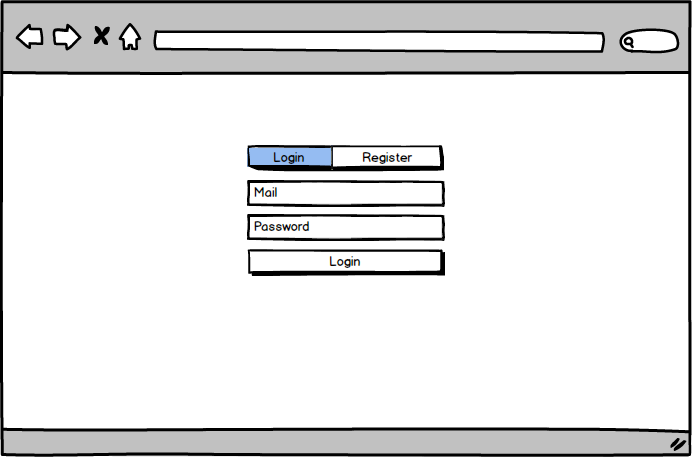
\includegraphics[width=0.7\linewidth]{kapitel1/mocks/Login.png}
 \caption{Login Screen Mock}
  \label{fig:login}
\end{figure}

\begin{figure}[h]
 \centering
 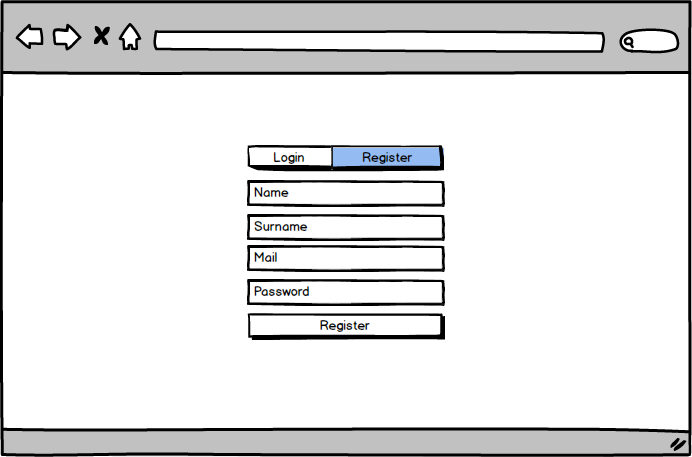
\includegraphics[width=0.7\linewidth]{kapitel1/mocks/Register.png}
 \caption{Register Screen Mock}
  \label{fig:register}
\end{figure}


\textbf{Login Formular}
\begin{itemize}
\item Mail (String, valide Mailadresse, eindeutig im System)
\item Password (String, mindestens 3 Zeichen, maximal 20 Zeichen)
\end{itemize}

\textbf{Register Formular}
\begin{itemize}
\item Name (String)
\item Surname (String)
\item Mail (String, valide Mailadresse, eindeutig im System)
\item Password (String, mindestens 3 Zeichen, maximal 20 Zeichen)
\end{itemize}



\subsubsection{System wählen / erstellen}

Da ein Nutzer in der Lage ist mehrere aktive Systeme zeitgleich zu monitoren,
wird eine Übersichtsseite (Abbildung \ref{fig:system-picker}) benötigt
um Systeme wechseln zu können. Zusätzlich sollen auf dieser Übersicht
neue Systeme angelegt werden können.

\begin{figure}[h]
 \centering
 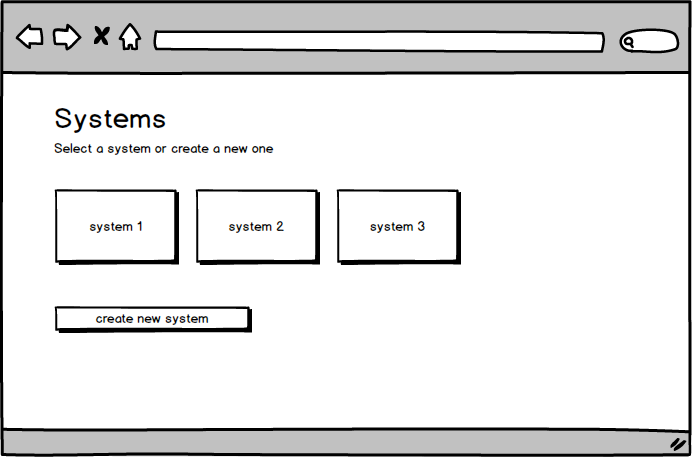
\includegraphics[width=0.6\linewidth]{kapitel1/mocks/system-picker.png}
 \caption{System wählen Mock}
 \label{fig:system-picker}
\end{figure}

\textbf{System erstellen}

\begin{itemize}
\item Name (String, maximal 20 Zeichen)
\item Beschreibung (String, maximal 255 Zeichen)
\end{itemize}


\subsubsection{Dashboard}

Auf dem Dashboard soll ein Nutzer die wichtigsten Informationen über sein System erhalten.
Fehlerverhalten des Systems soll deutlich und informativ dargestellt werden.
Zusätzlich soll das Dashboard als Einstiegspunkt für weitere Views dienen.

\subsubsection{Metriken}

Die Metriken Sektion soll pro Applikation eine Kollektion von Diagrammen beinhalten.
Dabei soll die Applikation, sowie der aktive Beobachtungszeitraum, gewählt werden können.

\begin{figure}[h]
 \centering
 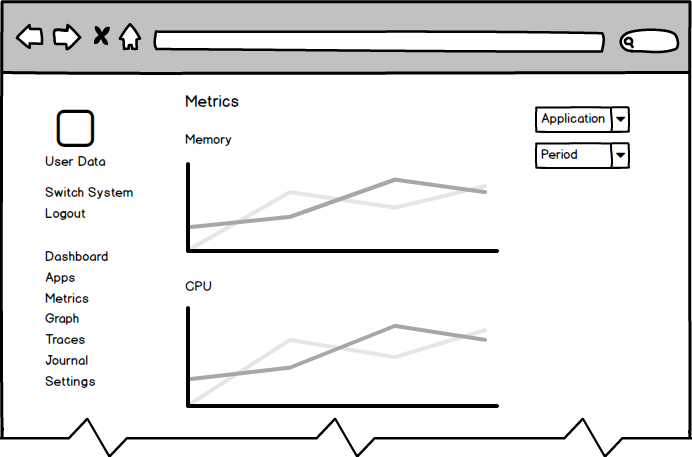
\includegraphics[width=0.6\linewidth]{kapitel1/mocks/metrics.png}
 \caption{Metrik Mock}
  \label{fig:metrics}
\end{figure}

\textbf{Diagramme}

\begin{itemize}
\item CPU Load
\item Memory
\item Requests client send
\item Requests server receive
\end{itemize}


\subsubsection{Graph}

Im Vergleich zur Metrik View soll der Graph nicht nur einzelne Applikationen darstellen,
sondern das Kommunikationsnetz des Gesamtsystems visualisieren.
Wie in Abbildung \ref{fig:graph} zu sehen ist, sollen dabei Services als Knoten und Requests als Kanten dargestellt werden.
Zu visualisierende Metriken sind Anzahl und Dauer der Requests zwischen den Services
Zusätzlich soll auch hier der Beobachtungszeitraum definiert werden können.

\begin{figure}[h]
 \centering
 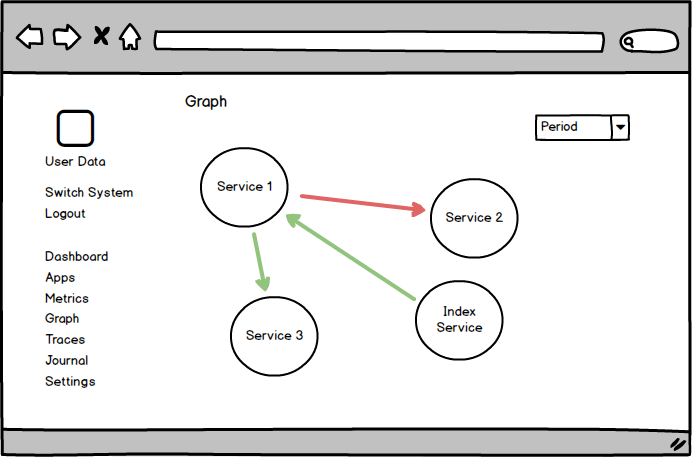
\includegraphics[width=0.6\linewidth]{kapitel1/mocks/graph.png}
 \caption{Graph Mock}
 \label{fig:graph}
\end{figure}

\subsubsection{Traces}

Die Traces Sektion besteht aus zwei Views. Einer Übersichtsliste der Request Einstiegspunkte,
welche zur Trace Detailseite (Abbildung \ref{fig:trace}) überleitet. Im Detail besteht ein Trace aus den Requests
aller an einer Aktion beteiligten Services. Dabei werden die Zeitlichen Abläufe in einem Gantt Chart dargestellt.

\begin{figure}[h]
 \centering
 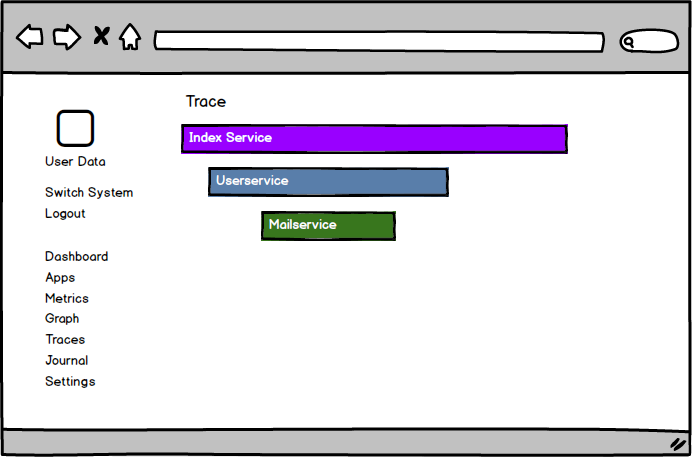
\includegraphics[width=0.6\linewidth]{kapitel1/mocks/trace.png}
 \caption{Trace Detailseite Mock}
 \label{fig:trace}
\end{figure}


\subsubsection{Journal}

Das Journal besteht aus Logeinträgen bezüglich Serverstart, Serverstop und Servercrash.

\begin{figure}[h]
 \centering
 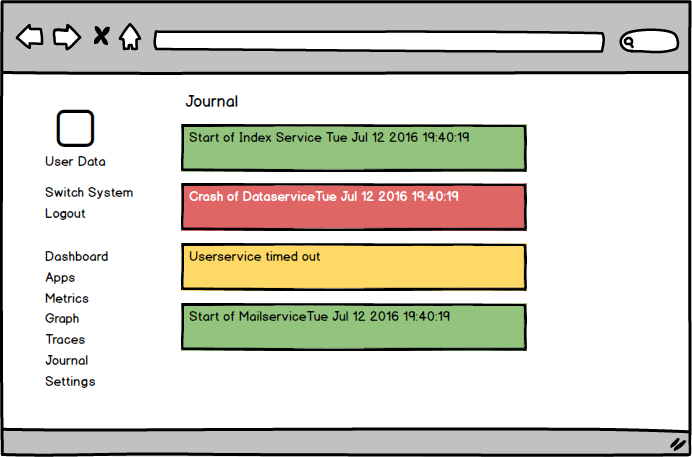
\includegraphics[width=0.6\linewidth]{kapitel1/mocks/journal.png}
 \caption{Journal Mock}
\end{figure}

\subsubsection{Settings}

In den Einstellungen können Nutzerrelevante Parameter definiert werden. Metadaten können geändert werden.
Nutzer sollen die Möglichkeit erhalten ein Profilbild einzustellen.

\subsubsection{Events}

Reaktiv werden Nutzer auf Fehlverhalten derer Applikationen hingewiesen. Sollten Services außerplahnmäßig terminieren oder ihre Erreichbarkeit verlieren,
wird dies als Event, also als Notification, für den User ausgegeben.

\textbf{Events}
\begin{itemize}
\item Service Start
\item Service Stop
\item Service Absturz
\item Anstieg von Request Latenzzeiten
\end{itemize}


\subsection{Plattformen}

Applikationen können anhand von Diagrammen und Graphen im Detail analysiert werden,
ferner möchte ein Nutzer reaktiv über Vorgänge seines Systems informiert werden, speziell wenn Latenzprobleme und Service-Ausfälle reibungslose Abläufe eines Systems gefährden.
Hierzu erhält der Nutzer Push Notifications über das Event System.

Die Applikation soll daher als App für iOS und Android, sowie als Desktop Applikation für MacOS, Linux und Windows zur Verfügung stehen.
In Anbetracht, dass das Frontend Team nur aus meiner Person besteht, stellt sich diese Anforderung, in der doch knappen Entwicklungszeit, als große Herausforderung dar.
Daher liegt die Entscheidung nahe, den Ansatz der hybriden App Entwicklung zu wählen, statt die Applikationen für die jeweilige Plattform nativ zu implementieren.
